\documentclass[DIV=15, 10pt]{scrartcl}

\usepackage{palatino}
\usepackage[ngerman]{babel}
\usepackage[T1]{fontenc}
\usepackage[utf8]{inputenc}
\usepackage{amsmath}
\usepackage{amssymb}
\usepackage{graphicx}
\usepackage{booktabs}

\setlength{\parindent}{0cm}
\setlength{\parskip}{3mm}

\newcommand{\PSet}{$\mathcal{P}$}
\newcommand{\KSet}{$\mathcal{K}$}

\begin{document}

\title{Schweizer Leiter und Kombinatorik}
\author{Dr. Volker Knollmann}

\maketitle

\begin{abstract}
Das Spielsystem "`Schweizer Leiter"' ist...  "dflsjdfk"
\end{abstract}

\section{Einleitung}

Dieser Artikel geht zunächst auf ein paar mathematisch-kombinatorische Grundlagen ein,
die für die nachfolgenden Betrachtungen des SL-Spielsystems erforderlich sind. Dazu
schauen wir zunächst ganz allgemein auf mögliche Kombinationen von Spielern und Spielrunden,
um daraus dann den Sonderfall "`Jeder-gegen-Jeden"' abzuleiten, der wiederum als Vorlage für
die nachfolgende Spezialisierung "`Schweizer Leiter"' ist.

Basierend auf diesem mathematischen Modell erläutert das Kapitel FIX, welche Herausforderungen
eine reale SL-Implementierung für eine Turnierverwaltung beherrschen muss. Besonderer Augenmerk
wird dabei auf stark variierenden Gruppengrößen von einigen wenigen bis einigen Dutzend
Teilnehmern liegen.

FIX: weitere Einführung

\subsection{Das Spielsystem "`Schweizer Leiter"'}

Im Kern handelt es sich bei SL um ein iteratives Spielsystem, in dem eine feste Anzahl Spieler eine in gewissen Grenzen frei wählbare Anzahl Runden spielt. Die Spielpaarungen für eine Runde ergeben sich aus einer Rangliste, die nach jeder Runde auf Basis eines Punktesystems und der Spielergebnisse aktualisiert wird.

Ein exemplarischer Turnierablauf ist in etwa wie folgt:

\begin{enumerate}

\item Vor Spielbeginn wird durch die Turnierleitung eine initiale Setzliste definiert, die allen Spielern eine initiale Platzierung zuordnet. Die initiale Platzierung kann beispielsweise zufällig gewählt oder, bei bekannten Spielern, auf Basis von Erfahrung, Ranglisten oder anderen Quellen abgeleitet werden.

\item Die Spielpaarungen ergeben sich als "`1. gegen 2."', "`3. gegen 4."', usw.

\item Die Spieler erhalten Punkte, beispielsweise zwei Punkte für einen Sieg und einen Punkt für ein Unentschieden (sofern ein Unentschieden zulässig ist).

\item Auf Basis der Punkte wird eine neue Rangliste erstellt. Spieler mit mehr Punkten (also mit mehr Siegen) erreichen höhere Plätze. Sollte das Teilnehmerfeld ungerade sein, kann alternativ auch der Quotient "`Punkte pro gespielte Runde"' herangezogen werden, um aussetzende Spieler nicht zu benachteiligen. Bei Punktgleichheit können sekundäre Kriterien für beispielsweise Satzdifferenz oder Punktedifferenz für die Bestimmung der Platzierung herangezogen werden.

\item Auf Basis der neuen Rangliste wird eine neue Runde gespielt; der Vorgang wiederholt sich ab (2) entsprechend.

\end{enumerate}

Die Anzahl der zu spielenden Runden kann die Turnierleitung weitestgehend frei festlegen. Das Turnierergebnis sind die Platzierungen nach der letzten Runde. Im Allgemeinen führen mehr Runden zu einem realistischerem Ergebnis. Typische Werte sind vier bis sechs Runden für übliche Teilnehmerfelder bis ca. 25 Teilnehmern.

Die Vorteile von SL:

\begin{itemize}

\item Alle Spieler bleiben im Turnier, kein Spieler scheidet aus.

\item Mit der Zeit spielen etwa gleich starke Gegner gegeneinander, was zu interessanteren Spielen führt.

\item Die Anzahl der zu spielenden Runden kann dynamisch dem Turnierverlauf angepasst werden.

\end{itemize}

Eine übliche Nebenbedingung bei der Definition der Spiele für die jeweils nächste Runde ist, dass \emph{Spielpaarungen sich nach Möglichkeit nicht wiederholen} sollen. Wenn im Laufe des Turniers beispielsweise die Begegnung "`3. gegen 4."' bereits in einer vorangegangenen Runde gespielt wurde, werden stattdessen die Begegnungen "`3. gegen 5."' und "`4. gegen 6."' angesetzt.

Natürlich kann es aber vorkommen, dass auch diese Alternativbegegnungen bereits gespielt wurden. Ein Schwerpunkt dieses Artikels wird sein, Strategien aufzuzeigen, wie mit einer derartigen Situation aus Sicht einer Turnierverwaltung (Software) umgegangen werden kann.

\subsection{Definitionen}

In den folgenden Abschnitten kommen die folgenden grundlegenden Symbole, Begriffe und Definitionen zur Anwendung:

\begin{description}

\item[Anzahl Spieler:] $n$

\item[Rundennummer:] $R_0$, $R_1$, $R_2$, ...

\item[Symbolische Spielernamen:] A, B, C, ...

\item[Rundenkonfiguration:] Die Liste der für eine Runde vorgesehenen Spielpaarungen

\item[Spielpaarungen:] A-B, B-E etc. bedeuten soviel wie "`A spielt gegen B"', "`B spielt gegen E"', usw.

\end{description}

Weitere Symbole werden im Laufe des Textes nach Bedarf eingeführt.

\section{Kombinatorische Grundlagen} 

Das Ziel dieses Abschnitts ist eine Herleitung der Anzahl der möglichen Rundenkonfigurationen im Turnier. Die Anzahl der Rundenkonfigurationen ist entscheidend dafür, ob das Nebenkriterium, Spielwiederholungen zu vermeiden, eingehalten werden kann.

Der Einfachheit halber gelte für alle nachfolgenden Betrachtungen:

\[
n \; \text{sei gerade}
\]

Diese Annahme ist ohne Beschränkung der Allgemeinheit zulässig, weil im Falle ungerader Spieleranzahlen mit einem zusätzlichen "`virtuellen"' Spieler gerechnet werden kann. Spiele gegen diesen virtuellen Spieler bedeuten dann ein Aussetzen des zugehörigen "`normalen"' Spielers.

\subsection{Allgemeine Betrachtungen}

Eine grundlegende Größe ist die Anzahl der Spielpaarungen, die für ein Feld von $n$ Spielern zur Verfügung steht. Diese Fragestellung entspricht der Suche nach den möglichen "`2-aus-$n$"'-Kombinationen -- ähnlich dem bekannten "`6-aus-49"' beim Lotto.

Bekanntermaßen berechnet sich die Anzahl solcher Kombinationen als Binomialkoeffizient, in diesem Falle als "'$n$-über-2"':

\begin{align*}
P &= \quad {{n}\choose{2}} \quad = \quad \frac{n!}{2! \; \cdot \; (n - 2)!} \quad
= \quad \frac{n!}{2 \; (n - 2)!} \nonumber \\[3mm]
&=\quad \frac{n \cdot (n - 1) \cdot (n - 2)!}{2 \; (n - 2)!} \quad = \quad
\frac{n(n-1)}{2}
\end{align*}

Beziehungsweise als Funktion:

\begin{equation}
P: \mathbb{N} \mapsto \mathbb{N}, \quad P(n) = \frac{n(n-1)}{2} \qquad
\text{für alle geraden }n \geq 2
\end{equation}

Die Menge dieser Spielpaarungen sei \PSet. Die Elemente von \PSet stellen gewissermaßen die "`Bausteine"' dar, aus denen die Rundenkonfigurationen aufgebaut werden können. Unter der Annahme einer geradzahligen Spieleranzahl $n$ besteht eine solche Rundenkonfiguration aus

\begin{equation}
N = \frac{n}{2}
\end{equation}

Spielen. Oder anders ausgedrückt: jede Rundenkonfiguration besteht aus einem $N$-Tupel  aus Spielpaarungen, von denen $P$ zur Auswahl stehen.

Soll die Anzahl der möglichen gültigen Rundenkonfigurationen bestimmt werden, ist zu berücksichtigen, dass jeder Spieler in jeder Runde nur einem Spiel zugeordnet werden darf. Spielt also beispielsweise bereits B-C, sind die Paarungen A-B, A-C oder C-A als weitere Spiele dieser Runde nicht zulässig.

Rein mathematisch bedeutet dies, dass für die die Wahl des ersten Spiels einer Runde $n$ Spieler zur Auswahl stehen. Für das zweite Spiel dann nur noch $n-2$ usw. Die Anzahl aller unter dieser Randbedingung definierbaren $N$-Tupel ergibt sich wiederum aus der Anwendung des Binomialkoeffizienten:

\begin{align}\label{eqnSizeOfKDash}
K' &= {{n}\choose{2}} \; \cdot \; {{n-2}\choose{2}} \; \cdot \;{{n-4}\choose{2}} \; \cdot \; \ldots
\; \cdot \; {{4}\choose{2}} \; \cdot \; {{2}\choose{2}}\nonumber \\[3mm]
&= \prod_{k = 0}^{N - 1}{{n - 2k}\choose{2}}
\end{align}

Diese Berechnung bestimmt die Gesamtanzahl aller möglichen $N$-Tupel von 2er-Paarungen, die sich aus einer $n$-elementigen Menge bilden lassen. Sie lässt unberücksichtigt, dass eine Rundenkonfiguration der Form "`A-B, C-D"' aus Turniersicht identisch ist mit "`C-D, A-B"'. Oder anders formuliert: sie zählt alle Permutationen der Elemente eines $N$-Tupels einzeln.

Um diesen Effekt herauszurechnen, muss $K'$ noch durch Anzahl der Permutationen jeder Rundenkonfiguration dividiert werden. Da die Anzahl der Permutationen eines $N$-Tupels $N!$ entspricht, ergibt sich somit die Zahl der gültigen Rundenkonfigurationen zu:

\begin{align}\label{eqnComplicated}
K \; &= \frac{1}{N!} \cdot \prod_{k=0}^{N-1}{{n-2k}\choose{2}} \nonumber\\[3mm]
&= \frac{1}{N!} \cdot \prod\frac{(n-2k)!}{2(n - 2k -2)!} \nonumber\\[3mm]
&= \frac{1}{N!} \cdot \prod\frac{(n-2k-2)! \cdot (n-2k-1)(n-2k)}{2(n-2k-2)!} \nonumber\\[3mm]
&= \frac{1}{N!} \cdot \prod\frac{(n-2k-1)(n-2k)}{2} \nonumber\\[3mm]
&= \frac{1}{2^N \cdot N!} \cdot \prod(n - 2k -1)(n - 2k) \nonumber\\[3mm]
&= \frac{\prod(n-2k)}{2^N \cdot N!} \cdot \prod_{k=0}^{N-1}(n - 2k -1)
\end{align}

Der erste Faktor in \eqref{eqnComplicated} entfällt, denn mit $n = 2N$ folgt, dass Zähler und Nenner des Bruchs identisch sind:

\begin{equation*}
\prod_{k=0}^{N-1}(2N - 2k) \; = \;
\prod_{k=0}^{N-1}2(N-k) \; = \;
2^N \cdot \prod_{k=0}^{N-1}(N-k) \; = \; 2^N \cdot N!
\end{equation*}

Die Anzahl gültiger Rundenkonfigurationen lässt sich also berechnen zu\footnote{Die Formel lässt sich auch "`intuitiv"' ableiten: der erste Spieler kann mit $n-1$ anderen Spieler kombiniert werden, der nächste nur noch mit $n-3$, der nächste mit $n-5$, usw.}

\begin{equation}\label{eqnSizeOfK}
K: \mathbb{N} \mapsto \mathbb{N}, \quad K(n) \; = \; \
\prod_{k=0}^{N-1}(n - 2k -1) \qquad \text{für alle geraden }N \geq 2
\end{equation}

Durch etwas anderes Auflösungen und Kürzen der Binomialkoeffizienten aus Gleichungen~\eqref{eqnSizeOfKDash} kann $K(n)$ auch in diese alternative Darstellung gebracht werden, die zwar "`kompakter"' aussieht, aber aufgrund der enthaltenen Fakultäten letztlich mehr Berechnungsaufwand erfordert:

\begin{equation}\label{eqnSizeOfK1}
K(n) \; = \; \frac{n!}{2^{n/2} \cdot N!} \quad = \quad \frac{n!}{2^{n/2} \cdot \left(\frac{n}{2}\right)!} \qquad \text{für alle geraden }N \geq 2
\end{equation}


Für die weitere Beschreibung sei die Menge aller gültigen Rundenkonfigurationen \KSet, wobei jedes Element von \KSet\ einem $N$-Tupel mit Elementen aus \PSet\ entspricht und jedes Tupel den oben skizzierten Regeln genügt.

Ein Planungsalgorithmus für Turniere kann grundsätzlich -- sofern keine Teilnehmer aus dem Turnier ausscheiden und $n$ somit im Turnierverlauf konstant bleibt -- aus diesen $K$ Rundenkonfigurationen wählen. Ein ganzes Turnier aus $r$ Runden besteht also aus einer Abfolge $R_0$, $R_1$, ... $R_{r-1}$ von \KSet -Elementen.

Soll für das Turnier die oben erwähnte Nebenbedindung gelten, dass sich keine Spielpaarungen im Turnierverlauf wiederholen dürfen, kann die Auswahl der Tupel nicht mehr frei erfolgen, sondern muss diese Nebenbedingung berücksichtigen.

\subsection{Algorithmische Bildung von \KSet}

Die Elemente von \KSet\ können durch einen rekursiven Algorithmus bestimmt werden. Nehmen wir dazu an, dass $S_0$, $S_1$, ..., $S_{n-1}$ $n$ Spieler bezeichnen. Die $N$-elementigen Tupel von \KSet\ können dann aus allen Spielpaarungen $S_0$:$S_1$, $S_0$:$S_2$, ..., $S_0$:$S_{n-1}$ kombiniert mit allen $(N-1)$-Tupeln der jeweils verbleibenden Spieler gebildet werden:

\[
\mathcal{K} = \left\lbrace
\begin{array}{ll}
S_0:S_1, & \{\text{alle Kombinationen von }S_2, S_3, \ldots, S_{n-1}\}\\
S_0:S_2, & \{\text{alle Kombinationen von }S_1, S_3, \ldots, S_{n-1}\}\\
S_0:S_3, & \{\text{alle Kombinationen von }S_1, S_2, \ldots, S_{n-1}\}\\
\cdots\\
S_0:S_{n-1}, & \{\text{alle Kombinationen von }S_1, S_2, \ldots, S_{n-2}\}\\
\end{array}
\right.
\]

Beziehungsweise als rekursive Funktion inklusive Abbruchkriterium:

\begin{equation}\label{AlgoK}
\begin{array}{rcl}
\mathcal{K}(S_0, S_1, S_2, \ldots, S{n_1}) & = & \left\lbrace
\begin{array}{ll}
S_0:S_1, \; \mathcal{K}(S_2, S_3, \ldots, S_{n-1})\\
S_0:S_2, \; \mathcal{K}(S_1, S_3, \ldots, S_{n-1})\\
S_0:S_3, \; \mathcal{K}(S_1, S_2, \ldots, S_{n-1})\\
\cdots\\
S_0:S_{n-1}, \; \mathcal{K}(S_1, S_2, \ldots, S_{n-2})\\
\end{array}\right.\\[12mm]
\mathcal{K}(S_0, S_1) & = & S_0 : S_1
\end{array}
\end{equation}

Eine Betrachtung der Mächtigkeit der auf diese Weise gebildeten \KSet\ zeigt, dass die nach o.~g. Algorithmus gebildeten Mengen vollständig sind.

Nach obiger Methode ergibt sich die Mächtigkeit von \KSet\ für $n$ Spieler als Anzahl der Kombinationen von $S_0$:$S_1$, $S_0$:$S_2$, ..., $S_0$:$S_{n-1}$ jeweils kombiniert mit der Mächtigkeit einer Menge von $n-2$ Spielern. Die Anzahl der Kombinationen von $S_0$:$S_1$, $S_0$:$S_2$, ..., $S_0$:$S_{n-1}$ beträgt genau $n-1$. Mithin gilt:

\begin{align}\label{eqnSizeOfK_Alt}
\lvert \mathcal{K}_n \rvert \; &= \; (n-1) \; \cdot \; \lvert \mathcal{K}_{n-2} \rvert \nonumber \\[3mm]
&= \; (n-1) \; \cdot \; (n - 3) \; \cdot \; \ldots \; \cdot \; 3 \; \cdot \; 1 \nonumber \\[3mm]
&= \; \prod_{k = 0}^{N -1}(n - 2k - 1) \qquad \text{mit }N = \frac{n}{2}
\end{align}

Dies ist identisch zu Gleichung~\eqref{eqnSizeOfK}.

Die Mächtigkeit der algorithmisch gebildeten Menge \KSet\ entspricht also der Anzahl der in Gleichung~\eqref{eqnSizeOfK} kombinatorisch abgeleiteten Anzahl der zulässigen Rundenkonfigurationen. Da sich die Rekursionsparameter immer in mindestens einem Element unterscheiden, können im Algorithmus auch keine unzuläassigen Permutationen an sich identischer Rundenkombinationen gebildet werden. Zusammen mit dem Nachweis der korrekten Mächtigkeit des gebildeten \KSet\ ist somit gezeigt, dass der Algorithmus \KSet\ vollständig bestimmt.

\subsection{Häufigkeit von Spielpaarungen}
\label{laHaeufigkeit}

Aus dem Algorithmus zur Bildung von \KSet\ in~\eqref{AlgoK} ist ersichtlich, dass bei $n$ Spielern jede Spielpaarung in $K(n-2)$ Rundenkombinationen vorkommt. Dies folgt auch nicht zuletzt daraus, dass nach Bildung einer Spielpaarung zwei Spieler festgelegt sind und daher nur noch $n-2$ für zugehörige Spielkombinationen zur Verfügung stehen. Und diese $n-2$ Spieler lassen sich zu $K(n-2)$ Paarungen kombinieren.

Umgekehrt kann eine bestimmte Kombination von $N-1$ Spielpaarungen nur genau einmal in \KSet\ enthalten sein, denn durch Festlegung von $N-1$ Spielpaarungen ist das letzte noch fehlende Element für ein vollständiges $N$-Tupel aus \KSet\ bereits implizit definiert, da \KSet\ frei von Wiederholungen und Permutationen ist.

Analog gilt:

\begin{itemize}

\item Jede Kombination von $N-2$ Spielpaarungen kommt $K(4) = 3$ mal in \KSet\ vor.

\item Jede Kombination von $N-3$ Spielpaarungen kommt $K(6) = 15$ mal in \KSet\ vor.

\item usw.
\end{itemize}

\subsection{Vermeidung von Mehrfachbegegnungen}

Sollen Mehrfachbegegnungen -- also die Wiederholung einer bereits gespielten Paarung -- strikt vermieden werden, schränkt dies die Wahlfreiheit der Rundenkonfigurationen und die Anzahl der spielbaren Runden ein.

Besteht jede Runde aus $N$ Spielen und stehen insgesamt $P$ Spielpaarungen zur Verfügung und soll jede Paarung nur einmal gespielt werden, so ergibt sich die erforderliche Rundenanzahl zu

\begin{align}
r_0 \quad &= \quad \frac{P}{N} \quad = \quad \frac{n(n-1)}{2} \cdot \frac{2}{n} \nonumber \\[3mm]
&= \quad n - 1
\end{align}

oder anders abgeleitet: jeder der $n$ Spieler kann maximal gegen $n-1$ andere Spieler antreten, wofür $n-1$ Spielrunden erforderlich sind.

Eine solche Sequenz von $n-1$ geeigneten Rundenkonfigurationen muss existieren. \KSet\ enthält alle Kombinationen aller Spielpaarungen und in jeder der $n-1$ Runden wird eine neue Kombination von $N$ bisher nicht verwendeten Paarungen gespielt, für die es genau ein $N$-Tupel in \KSet\ gibt. Eine derartige Rundenabfolge ist auch als "`Jeder-gegen-Jeden"' bekannt.

Umgekehrt führt \emph{nicht} jede frei gewählte Sequenz von Rundenkonfigurationen automatisch zu einem vollständigen "`Jeder-gegen-Jeden"'-Durchgang. Ein Beispiel für einen solchen Fall ist in Abbildung~\ref{figDeadlock} dargestellt. Die Matrix enthält in ihren Spalten alle Rundenkonfigurationen für ein 6er-Teilnehmerfeld. Jede Spalte repräsentiert also ein 3-Tupel von Spielpaarungen aus \KSet. Die Zeilen stehen entsprechend für die jeweiligen Spielpaarungen in einer Runde.

\begin{figure}[hbtp]
\centering
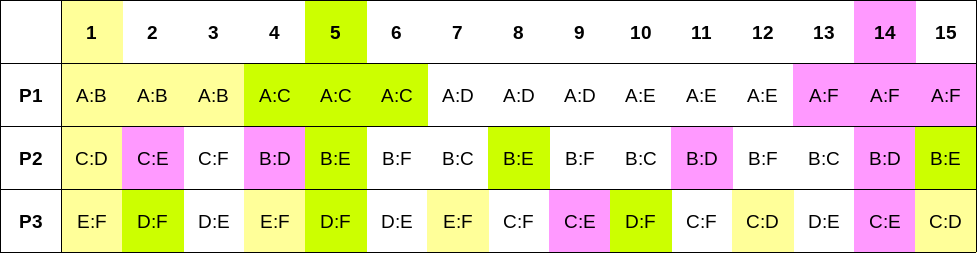
\includegraphics[width=0.8\textwidth]{Verklemmung6_6er.png}
\caption{Verklemmung in einem 6er-Feld}
\label{figDeadlock}
\end{figure}

In dem gezeigten Beispiel wurde in der ersten Runde die Konfiguration~1 gespielt. Die zugehörigen Begegnungen sind A:B, C:D und E:F (gelb hervorgehoben). Durch das Spielen dieser Begegnungen stehen nach Runde~1 alle Rundenkonfigurationen, die eine dieser Spielpaarungen enthalten, nicht mehr für den weiteren Turnierablauf zur Verfügung. Ansonsten würde die Regel zur Vermeidung von Mehrfachbegegnungen verletzt.

Für die zweite Runde wurde (willkürlich) Konfiguration~5 gewählt (grün). Diese Wahl war legitim, weil Konfiguration~5 keine der bereits gespielten Paarungen enthält. Entsprechend wurde für Runde~3 auf Konfiguration~14 zurückgegriffen (pink).

Wie Abbildung~\ref{figDeadlock} zeigt, steht nach Abschluss der dritten Runde keine Rundenkonfiguration mehr zur Verfügung, die nicht wenigstens eine bereits gespielte Paarung enthält. Ein Weiterspielen unter Vermeidung von Mehrfachbegegnungen ist also nicht möglich, obwohl noch nicht alle Spielpaarungen ausgespielt wurden. Die ungeschickte Wahl der Abfolge der Rundenkonfigurationen hat zu einer "`Verklemmung"' geführt.

Mittels Durchrechnen aller möglichen Spielabfolgen kann gezeigt werden, dass es für den oben gezeigten Fall $n=6$ insgesamt 120 Sequenzen gibt, die nach der dritten Runde zu einer Verklemmung führen. Dem stehen 720 Sequenzen gegenüber, mit denen sich alle fünf erforderlichen Runden konfliktfrei durchspielen lassen.

Ebenso kann für $n=8$ gezeigt werden, dass es nach der fünften Runde zu zahlreichen Verklemmungen kommt. Genauer gibt es zu jeder Erstrundenkonfiguration 27648 Sequenzen, die zu einer Verklemmung nach Runde fünf führen. Bei $K(8) = 105$ möglichen Erstrundenkonfigurationen ergeben sich mithin 2.903.040 ungültige Rundensequenzen. Die Zahl der gültigen Sequenzen bis Turnierende beträgt 31.449.705.

Wird mit den gültigen Sequenzen weitergespielt, kommt es weder bei $n=6$ noch bei $n=8$ zu weiteren Verklemmungen. Ebenso sind für $n=4$ grundsätzlich alle Sequenzen verklemmungsfrei. Tabelle~\ref{tabDeadlock} fasst die Ergebnisse zusammen und setzt auch die gültigen Sequenzen bis zur Verklemmungsrunde mit den ungültigen Sequenzen ins Verhältnis.

\begin{table}[htbp]
\begin{center}
\begin{tabular}{cccccc}
\toprule
$\quad n \quad$ & Runden & Verklemmung & Gültige Seq. & Ungültige Seq. & Verhältnis\\
& zu spielen & nach Runde & bis Verklemmung & bis Verklemmung & gültig : ungültig\\[1mm]
\midrule
4 &  3 &  -- & -- & -- & -- \\[1mm]
6 &  5 &  3 & 375 & 120 & 3,125 \\[1mm]
8 &  7 &  5 & 13.608.105 & 2.903.040 & ca. 4,7 \\[1mm]
\midrule
10 & 9 & 7\\[1mm]
12 & 11 & 9\\[1mm]
14 & 13 & 11\\[1mm]
\bottomrule
\end{tabular}
\caption{Mögliche Verklemmungen für $n=4, \; 6, \; 8$ (vollständig) und $n=10, \; 12, \; 14$ (Stichproben)}
\label{tabDeadlock}
\end{center}
\end{table}

Ergänzend enthält Tabelle~\ref{tabDeadlock} noch stichprobenartig bestimmte Verklemmungen für einige $n > 8$. Zur Verringerung der numerischen Komplexität wurde bis zum Bereich der vermuteten Runde, bei der eine Verklemmung auftritt (Runde $n-3$), unter Verzicht auf Testen aller Kombinationen gerechnet und einfach nur eine exemplarische Sequenz bestimmt. Ab da wurden dann alle weiteren Runden mit unter Anwendung aller verbleibenden Kombinationen durchprobiert. Zur Absicherung der Ergebnisse wurde die Einzelsequenz nicht nur bis zur vermuteten "`Verklemmungsrunde"' gerechnet, sondern bereits eine Runde vorher abgebrochen und entsprechend mit dem Durchprobieren der Kombinationen fortgeführt.

In jedem Falle zeigte sich eine Verklemmung nur bei Runde $n-3$. Verklemmung in früheren oder späteren Runden konnten weder im Stichprobenverfahren ($n > 8$) noch bei Durchprobieren aller Kombinationen ($n \leq 8$) festgestellt werden.

Obwohl die gezeigten Stichproben kein Beweis im mathematischen Sinne sind, liegt doch die Vermutung nahe, dass es bei jeder Spieleranzahl zu Verklemmungen kommen kann, auch wenn

\begin{itemize}

\item die Wahrscheinlichkeit für eine Verklemmung bei Wahl einer zufälligen Sequenz von Rundenkonfigurationen bei zunehmenden $n$ eher geringer wird; und

\item Verklemmungen überhaupt nur bei $n > 4$ und bei Runde $n - 3$ aufzutreten scheinen.

\end{itemize}

\minisec{Freie Rundenkonfigurationen nach Runden}

Eng verwandt mit dem Phänomen der Verklemmung ist die Frage nach der Anzahl noch verfügbarer Rundenkonfigurationen bei zunehmender Anzahl gespielter Runden. Eine Rundenkonfiguration gilt dabei als "`verfügbar"', wenn noch keine der enthaltenen Spielpaarungen gespielt wurde.

Eine genaue Berechnung ist leider nur für die freien Konfigurationen nach der ersten Runde möglich. Die Berechnung führt über die Kalkulation der Rundenkonfigurationen, die mindestens eine gespielte Paarung enthalten:

\begin{itemize}

\item Bei $n$ Spielern und $N = \frac{n}{2}$ Spielen pro Runde gibt es nach der ersten Runde genau eine Rundenkonfiguration, die $N$ gespielte Paarungen enthält (eben genau die gespielte Runde).

\item Eine Rundenkonfiguration mit $N-1$ gespielten Paarungen kann es nach der ersten Runde nicht geben. $N-1$ Paarungen legen genau ein $N$-Tupel fest, weil sich das $N$. Element im Tupel aufgrund des Fehlens von Wiederholungen und Permutationen in \KSet\ zwingend ergibt. Das Tupel mit $N$ gespielten Paarungen ist allerdings bereits berücksichtigt (s.~o.).

\item Es gibt $k_{N-2} = {N\choose{N-2}} = \frac{1}{2} \cdot N(N-1)$ Kombinationen von $N-2$ Spielpaarungen aus den $N$ gespielten Paarungen. Jede diese Kombinationen kommt $K(4) = 3$ mal vor (siehe auch Abschnitt~\ref{laHaeufigkeit}). Von diesen $3k_{N-2}$ Kombinationen stecken allerdings ${N\choose{N-2}}$ Kombinationen bereits in der gespielten Rundenkonfiguration aus $N$ Paarungen. Es verbleiben also $2k_{N-2} = N(N-1)$ Paarkombinationen, die sich auf andere Rundenkonfigurationen verteilen.

\item Es gibt $k_{N-3} = {N\choose{N-3}} = \frac{1}{6} \cdot N(N-1)(N-2) =
\frac{1}{3} (N-2) k_{N-2}$ Kombinationen von $N-3$ Spielpaarungen aus den $N$ gespielten Paarungen. Jede diese Kombinationen kommt $K(6) = 15$ mal vor. Von diesen $15k_{N-3}$ Kombinationen sind allerdings abzuziehen:

\begin{itemize}

\item ${N\choose{N-3}}$ Paarkombinationen, die in der gespielten Rundenkonfiguration enthalten sind; und

\item ${{N-2}\choose{N-3}} = N-2$ Paarkombinationen, die bereits in vorher berechneten $(N-2)$-Tupel von Spielpaarungen enthalten sind.
\end{itemize}

\item Und so weiter, bis schließlich die Anzahl der Rundenkonfigurationen mit nur einer Paarbelegung bestimmt wird.

\item Die Subtraktion der Summe aller Rundenkonfigurationen mit "`benutzten"' Spielpaarungen von der Gesamtzahl der Rundenkonfiguration ergibt schließlich die Anzahl der verfügbaren Rundenkonfigurationen für die zweite Runde.

\end{itemize}

Beispiel für $n=12$ mit $N=6$:

\begin{itemize}

\item Es gibt $K(12) = 10395$ mögliche Rundenkonfigurationen und $P(12) = 132$ Spielpaarungen. Jede Rundenkonfigurationen besteht aus $N$ -- also sechs -- dieser 132 Paarungen.

\item Nach der ersten Runde sind sechs von 132 Paarungen gespielt.

\item Es gibt genau eine Rundenkonfiguration, in der alle sechs Paarungen den sechs gespielten Paarungen entspricht: $k_6 = 1$.

\item Es kann keine Rundenkonfiguration mit fünf gespielten Paarungen geben: $k_5 = 0$.

\item Aus sechs gespielten Paarungen können ${6\choose4} = 15$ Kombinationen zu je vier Paarungen gebildet werden. Jede 4er-Kombination von Paaren ist dreimal in \KSet\ enthalten, was also $45$ 4er-Kombinationen der gespielten sechs Paarungen in \KSet\ entspricht. Davon sind allerdings $15$ Kombinationen bereits in der gespielten 6er-Kombination enthalten. Somit verbleiben $30$ Rundenkonfigurationen mit einer Belegung von jeweils vier der sechs enthaltenen Paarungen: $k_4 = 45 - k_6 \cdot 15 = 30$.

\item Aus sechs gespielten Paarungen können ${6\choose3} = 20$ Kombinationen zu je drei Paarungen gebildet werden. Jede 3er-Kombinationen von Paaren ist 15-mal in \KSet\ enthalten, was also 300 3er-Kombinationen entspricht. Davon sind allerdings $20$ Kombinationen bereits in der gespielten 6er-Paarung enthalten. Außerdem sind ${4\choose3} = 4$ 3er-Kombinationen in jeder der $30$ 4er-Paarungen enthalten. Die Anzahl der Rundenkonfigurationen mit genau drei gespielten Paarungen ist daher: $k_3 = 300 - k_6\cdot20 - k_4 \cdot 4 = 300 - 20 - 120 = 160$.

\item Analog lassen sich $k_2$ zu $900$ und $k_1$ zu $3264$ bestimmen.

\item Die Anzahl der Rundenkonfigurationen ohne jede gespielte Paarung beträgt daher zu Beginn der zweiten Runde: $k_{\text{frei}} = K(12) - \sum_{i=1}^6{k_i} = 6040$.

\end{itemize}

Die Anzahl der freien Rundenkonfigurationen nach Runde $2, \; 3, \ldots \;$ ist nicht mehr konstant und hängt von der gewählten Sequenz der Rundenkonfigurationen ab. Das drückt sich nicht zuletzt dadurch aus, dass einige Sequenzen zu einer Verklemmung führen (s.~o.) -- also zu $0$ freien Rundenkonfigurationen --, während andere Sequenzen verklemmungsfrei bis zur $n-1$. Runde führen.

Eine Berechnung aller Kombinationen für einige $n$ ist in Tabelle~\ref{tabFreeCount} aufgeführt. In erster Näherung zeigt sich eine Halbierung der verfügbaren Rundenkonfigurationen nach jeder Spielrunde, sofern mit verklemmungsfreien Sequenzen gearbeitet wird (Tabelle~\ref{tabFreeCountRel}). Zusammen mit der oben erläuterten Methode zur Berechnung der freien Konfigurationen nach der ersten Runde kann somit die ungefähre Anzahl freier Konfigurationen zu Beginn jeder Spielrunde abgeschätzt werden.

\begin{table}[htbp]
\begin{center}
\begin{tabular}{ccccccc}
\toprule
$\quad n \quad$ & $K(n)$ & frei nach & frei nach & frei nach & frei nach & frei nach\\
&& Runde 1 & Runde 2 & Runde 3 & Runde 4 & Runde 5\\[1mm]
\midrule
4 & 3 & 2 & 1 & 0 & -- & --\\[1mm]
6 & 15 & 8 & 4 & 2 & 1 & 0\\[1mm]
8 & 105 & 60 & 31 \ldots 33 & 14 \ldots 24 & 5 \ldots 9 & 2 \ldots 4\\[1mm]
10 & 945 & 544 & 292 \ldots 293 & 142 \ldots 146\\[1mm]
12 & 10395 & 6040 & 3326 \ldots 3329\\[1mm]
\bottomrule
\end{tabular}
\caption{Freie Rundenkonfigurationen nach Spielerzahl und Runde (absolut)}
\label{tabFreeCount}
\end{center}
\end{table}

\begin{table}[htbp]
\begin{center}
\begin{tabular}{ccccccc}
\toprule
$\quad n \quad$ & $K(n)$ & frei nach & frei nach & frei nach & frei nach & frei nach\\
&& Runde 1 & Runde 2 & Runde 3 & Runde 4 & Runde 5\\[1mm]
\midrule
4 & 3 & 0,66 & 0,5 & n/a & -- & --\\[1mm]
6 & 15 & 0,53 & 0,5 & 0,5 & 0,5 & n/a\\[1mm]
8 & 105 & 0,57 & 0,53 & 0,42 \ldots 0,75 & 0,2 \ldots 0,64 & 0,22 \ldots 0,8\\[1mm]
10 & 945 & 0,58 & 0,54 & 0,49\\[1mm]
12 & 10395 & 0,58 & 0,55\\[1mm]
\bottomrule
\end{tabular}
\caption{Freie Rundenkonfigurationen nach Spielerzahl und Runde (relativ zur Vorrunde)}
\label{tabFreeCountRel}
\end{center}
\end{table}

\section{Anwendung auf "`Schweizer Leiter"'}

\subsection{Allgemeines}

Wie eingangs ausgeführt werden bei SL die Spielpaarungen nach dem Prinzip "`1. gegen 2."', "`3. gegen 4."' etc. gebildet, wobei die Platzierungen nach jeder Spielrunde nach einem Punktesystem neu berechnet werden.

Da die Spielergebnisse nicht vorhersagbar sind, liegt bei der Bestimmung der Spielpaarungen der nächsten Runde prinzipiell eine zufällige Auswahl einer Rundenkonfiguration aus \KSet\ vor. Wie im vorangegangenen Abschnitt erläutert ist dieses Vorgehen mit zwei grundsätzlichen Problemen verbunden, sofern Mehrfachbegegnungen vermieden werden sollen:

\begin{enumerate}

\item Eine oder mehrere der gebildeten Spielpaarungen wurde(n) bereits in einer vorangegangenen Runde gespielt, so dass eine alternative Rundenkonfiguration gebildet werden muss.

\item Manche Spielsequenzen führen zu Verklemmungen, die ein Weiterführen ohne Mehrfachbegegnungen unmöglich machen.

\end{enumerate}

Das erste Problem führt dazu, dass mitunter die erforderliche Kombination von Paarungen nicht verfügbar ist und auf eine andere Paarung ausgewichen werden muss. Das zweite Problem verursacht, dass \emph{gar keine} weitere Runde gespielt werden kann.

Im Idealfall konvergiert SL mit $n$ Teilnehmern nach $n-1$ Runden gegen ein "`Jeder-gegen-Jeden"'. Daher ist ein SL-Turnier auf jeden Fall nach $n-1$ Runden beendet, sofern Mehrfachbegegnungen ausgeschlossen wurden.

\minisec{Bildung wiederholungsfreier Rundenkonfigurationen}

Führt das nach dem Prinzip "`1. gegen 2."', "`3. gegen 4."', ... gebildete Tupel von Spielpaarungen zu einer Kollision mit vorangegangenen Spielpaarungen, muss die Bildung der Spielpaarungen modifiziert werden.

Hat beispielweise das Spiel "`7. gegen 8."' bereits stattgefunden, kann alternativ auf  "`7. gegen 9."' in Kombination mit "`8. gegen 10."' ausgewichen werden. Kann auf diese Weise kein geeigneter Gegner gefunden werden, muss ggf. eine vorangegangene Paarung verändert werden.

Eine algorithmische Umsetzung kann in etwa so erfolgen ($S_x$ bezeichnet den aktuell an Platz $x$ stehenden Spieler):

\begin{enumerate}

\item Starte mit $i = 1$. Solange $i < n$:

\item Starte mit $k = i + 1$. Inkrementiere $k$ bis zu einer Spielpaarung $S_i$:$S_k$, die noch nicht in einer vorangegangenen Runde gespielt wurde. Merke $S_k$ als nächsten Gegner für $S_i$ vor. Merke $S_i$ und $S_k$ als für die nächste Runde verplant vor.

\item Kann kein geeignetes $k$ gefunden werden, lösche die zuletzt getroffen Spielerpaarung und setze mit dem zugehörigen $i$ und einem zugehörigen $k+1$ bei im Schritt (2) fort.

\item Inkrementiere $i$ bis $S_i$ einen noch nicht verplanten Spieler bezeichnet oder $i = n$ ist.

\item Ist $i < n$ fahre mit Schritt (3) fort. Ist $i = n$ und sind noch nicht alle Spieler verplant, verfahre wie in Schritt (3).

\end{enumerate}

Diese Algorithmus bildet eine gültige Rundenkonfiguration aus noch nicht gespielten Paarungen, sofern keine Verklemmung vorliegt (die Erkennung der Verklemmung ist in dem oben skizzierten Algorithmus nicht enthalten).

\minisec{Umgang mit Verklemmungen}



\end{document}

